\documentclass{standalone}
\usepackage{tikz}
\usetikzlibrary{patterns}
\usetikzlibrary{positioning}
\usetikzlibrary{patterns, positioning}
\usetikzlibrary{shapes.misc}
\usepackage[outline]{contour}
\contourlength{1.5pt} 
\usetikzlibrary{calc}
        \usepackage{relsize}
        \tikzset{fontscale/.style = {font=\relsize{#1}}}

\begin{document}
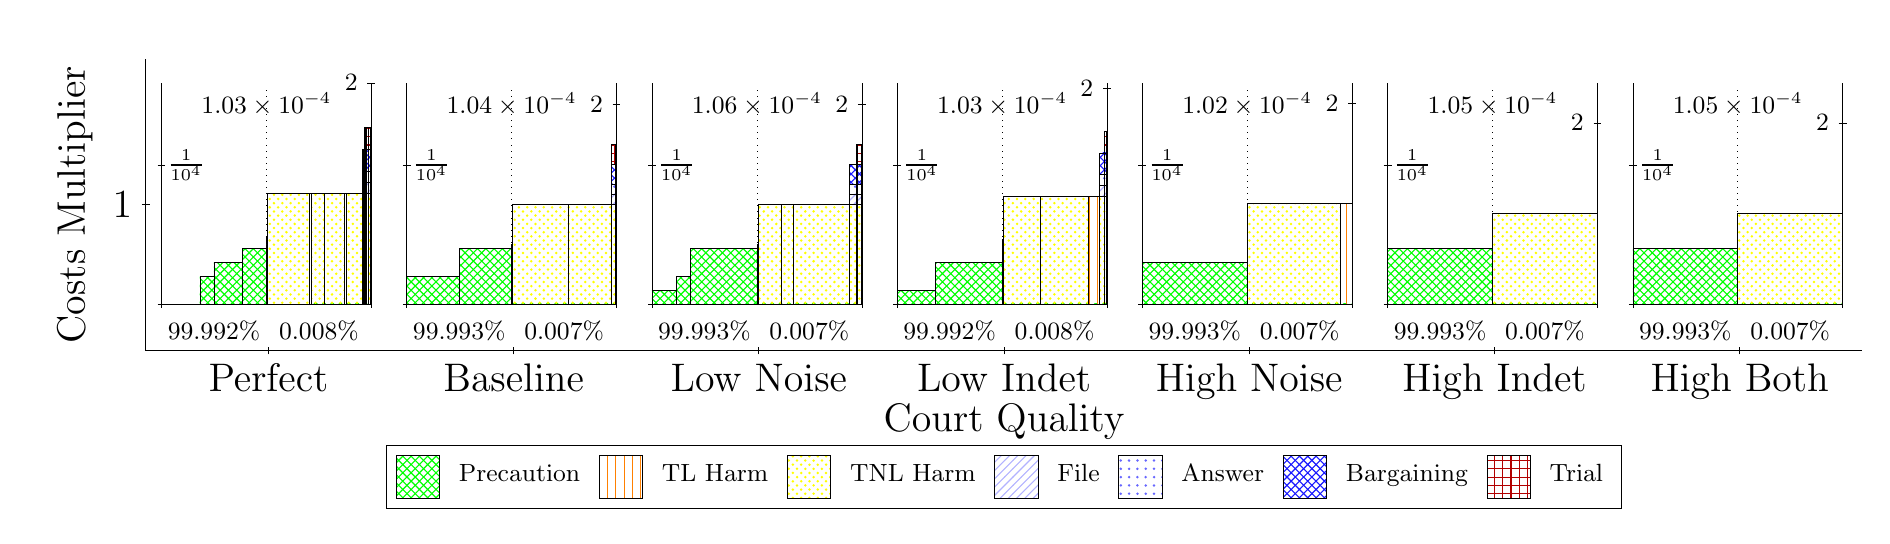
\begin{tikzpicture}
\clip(-0.5,-1.1) rectangle +(23.3,6.2);
\draw[black] (1,1) -- (1,4.7);
\node[rotate=90, fontscale=2, anchor=center] at (0.1, 2.85) {Costs Multiplier};
\draw[black] (0.95,2.85) -- (1.05,2.85);
\node[fontscale=2, anchor=east] at (0.95, 2.85) {1};

\draw[black] (1,1) -- (22.8,1);
\node[fontscale=2, anchor=center] at (11.9, 0.1) {Court Quality};
\draw[black] (2.5571,0.95) -- (2.5571,1.05);
\node[fontscale=2, anchor=north] at (2.5571, 0.95) {Perfect};
\draw[black] (5.6714,0.95) -- (5.6714,1.05);
\node[fontscale=2, anchor=north] at (5.6714, 0.95) {Baseline};
\draw[black] (8.7857,0.95) -- (8.7857,1.05);
\node[fontscale=2, anchor=north] at (8.7857, 0.95) {Low Noise};
\draw[black] (11.9,0.95) -- (11.9,1.05);
\node[fontscale=2, anchor=north] at (11.9, 0.95) {Low Indet};
\draw[black] (15.014,0.95) -- (15.014,1.05);
\node[fontscale=2, anchor=north] at (15.014, 0.95) {High Noise};
\draw[black] (18.129,0.95) -- (18.129,1.05);
\node[fontscale=2, anchor=north] at (18.129, 0.95) {High Indet};
\draw[black] (21.243,0.95) -- (21.243,1.05);
\node[fontscale=2, anchor=north] at (21.243, 0.95) {High Both};


\draw[pattern=crosshatch, pattern color=green,draw=black,very thin] (1.6864,1.592) rectangle (1.8661,1.9441);
\draw[pattern=crosshatch, pattern color=green,draw=black,very thin] (1.8661,1.592) rectangle (2.2257,2.1201);
\draw[pattern=crosshatch, pattern color=green,draw=black,very thin] (2.2257,1.592) rectangle (2.5321,2.2961);
\draw[pattern=north east lines, pattern color=blue!30,draw=black,very thin] (2.5321,1.592) rectangle (2.5338,1.7324);
\draw[pattern=dots,  pattern color=blue!60,draw=black,very thin] (2.5321,1.7324) rectangle (2.5338,1.8728);
\draw[pattern=crosshatch,      pattern color=blue!90,draw=black,very thin] (2.5321,1.8728) rectangle (2.5338,2.1536);
\draw[pattern=north east lines, pattern color=blue!30,draw=black,very thin] (2.5338,1.592) rectangle (2.5371,1.7324);
\draw[pattern=dots,  pattern color=blue!60,draw=black,very thin] (2.5338,1.7324) rectangle (2.5371,1.8728);
\draw[pattern=crosshatch,      pattern color=blue!90,draw=black,very thin] (2.5338,1.8728) rectangle (2.5371,2.1536);
\draw[pattern=grid,            pattern color=red!70!black,draw=black,very thin] (2.5338,2.1536) rectangle (2.5371,2.4344);
\draw[pattern=crosshatch, pattern color=green,draw=black,very thin] (2.5371,1.592) rectangle (2.54,1.592);
\draw[pattern=north east lines, pattern color=blue!30,draw=black,very thin] (2.5371,1.592) rectangle (2.54,1.7324);
\draw[pattern=dots,  pattern color=blue!60,draw=black,very thin] (2.5371,1.7324) rectangle (2.54,1.8728);
\draw[pattern=crosshatch,      pattern color=blue!90,draw=black,very thin] (2.5371,1.8728) rectangle (2.54,2.1536);
\draw[pattern=grid,            pattern color=red!70!black,draw=black,very thin] (2.5371,2.1536) rectangle (2.54,2.4344);
\draw[pattern=crosshatch, pattern color=green,draw=black,very thin] (2.54,1.592) rectangle (2.5458,1.592);
\draw[pattern=north east lines, pattern color=blue!30,draw=black,very thin] (2.54,1.592) rectangle (2.5458,1.7324);
\draw[pattern=dots,  pattern color=blue!60,draw=black,very thin] (2.54,1.7324) rectangle (2.5458,1.8728);
\draw[pattern=crosshatch,      pattern color=blue!90,draw=black,very thin] (2.54,1.8728) rectangle (2.5458,2.1536);
\draw[pattern=grid,            pattern color=red!70!black,draw=black,very thin] (2.54,2.1536) rectangle (2.5458,2.4344);
\draw[pattern=crosshatch dots, pattern color=yellow,draw=black,very thin] (2.5458,1.592) rectangle (3.0769,2.996);
\draw[pattern=vertical lines, pattern color=orange,draw=black,very thin] (3.0769,1.592) rectangle (3.1059,2.996);
\draw[pattern=crosshatch, pattern color=green,draw=black,very thin] (3.1059,1.592) rectangle (3.2629,1.592);
\draw[pattern=crosshatch dots, pattern color=yellow,draw=black,very thin] (3.1059,1.592) rectangle (3.2629,2.996);
\draw[pattern=crosshatch, pattern color=green,draw=black,very thin] (3.2629,1.592) rectangle (3.2676,1.592);
\draw[pattern=vertical lines, pattern color=orange,draw=black,very thin] (3.2629,1.592) rectangle (3.2676,2.996);
\draw[pattern=crosshatch, pattern color=green,draw=black,very thin] (3.2676,1.592) rectangle (3.5213,1.592);
\draw[pattern=crosshatch dots, pattern color=yellow,draw=black,very thin] (3.2676,1.592) rectangle (3.5213,2.996);
\draw[pattern=crosshatch, pattern color=green,draw=black,very thin] (3.5213,1.592) rectangle (3.5414,1.592);
\draw[pattern=vertical lines, pattern color=orange,draw=black,very thin] (3.5213,1.592) rectangle (3.5414,2.996);
\draw[pattern=crosshatch, pattern color=green,draw=black,very thin] (3.5414,1.592) rectangle (3.7548,1.5921);
\draw[pattern=crosshatch dots, pattern color=yellow,draw=black,very thin] (3.5414,1.5921) rectangle (3.7548,2.996);
\draw[pattern=crosshatch dots, pattern color=yellow,draw=black,very thin] (3.7548,1.592) rectangle (3.7633,2.996);
\draw[pattern=north east lines, pattern color=blue!30,draw=black,very thin] (3.7548,2.996) rectangle (3.7633,3.1364);
\draw[pattern=dots,  pattern color=blue!60,draw=black,very thin] (3.7548,3.1364) rectangle (3.7633,3.2768);
\draw[pattern=crosshatch,      pattern color=blue!90,draw=black,very thin] (3.7548,3.2768) rectangle (3.7633,3.5576);
\draw[pattern=vertical lines, pattern color=orange,draw=black,very thin] (3.7633,1.592) rectangle (3.7718,2.996);
\draw[pattern=north east lines, pattern color=blue!30,draw=black,very thin] (3.7633,2.996) rectangle (3.7718,3.1364);
\draw[pattern=dots,  pattern color=blue!60,draw=black,very thin] (3.7633,3.1364) rectangle (3.7718,3.2768);
\draw[pattern=crosshatch,      pattern color=blue!90,draw=black,very thin] (3.7633,3.2768) rectangle (3.7718,3.5576);
\draw[pattern=crosshatch dots, pattern color=yellow,draw=black,very thin] (3.7718,1.592) rectangle (3.7882,2.996);
\draw[pattern=north east lines, pattern color=blue!30,draw=black,very thin] (3.7718,2.996) rectangle (3.7882,3.1364);
\draw[pattern=dots,  pattern color=blue!60,draw=black,very thin] (3.7718,3.1364) rectangle (3.7882,3.2768);
\draw[pattern=crosshatch,      pattern color=blue!90,draw=black,very thin] (3.7718,3.2768) rectangle (3.7882,3.5576);
\draw[pattern=grid,            pattern color=red!70!black,draw=black,very thin] (3.7718,3.5576) rectangle (3.7882,3.8384);
\draw[pattern=vertical lines, pattern color=orange,draw=black,very thin] (3.7882,1.592) rectangle (3.8046,2.996);
\draw[pattern=north east lines, pattern color=blue!30,draw=black,very thin] (3.7882,2.996) rectangle (3.8046,3.1364);
\draw[pattern=dots,  pattern color=blue!60,draw=black,very thin] (3.7882,3.1364) rectangle (3.8046,3.2768);
\draw[pattern=crosshatch,      pattern color=blue!90,draw=black,very thin] (3.7882,3.2768) rectangle (3.8046,3.5576);
\draw[pattern=grid,            pattern color=red!70!black,draw=black,very thin] (3.7882,3.5576) rectangle (3.8046,3.8384);
\draw[pattern=crosshatch, pattern color=green,draw=black,very thin] (3.8046,1.592) rectangle (3.8198,1.592);
\draw[pattern=crosshatch dots, pattern color=yellow,draw=black,very thin] (3.8046,1.592) rectangle (3.8198,2.996);
\draw[pattern=north east lines, pattern color=blue!30,draw=black,very thin] (3.8046,2.996) rectangle (3.8198,3.1364);
\draw[pattern=dots,  pattern color=blue!60,draw=black,very thin] (3.8046,3.1364) rectangle (3.8198,3.2768);
\draw[pattern=crosshatch,      pattern color=blue!90,draw=black,very thin] (3.8046,3.2768) rectangle (3.8198,3.5576);
\draw[pattern=grid,            pattern color=red!70!black,draw=black,very thin] (3.8046,3.5576) rectangle (3.8198,3.8384);
\draw[pattern=crosshatch, pattern color=green,draw=black,very thin] (3.8198,1.592) rectangle (3.8265,1.592);
\draw[pattern=vertical lines, pattern color=orange,draw=black,very thin] (3.8198,1.592) rectangle (3.8265,2.996);
\draw[pattern=north east lines, pattern color=blue!30,draw=black,very thin] (3.8198,2.996) rectangle (3.8265,3.1364);
\draw[pattern=dots,  pattern color=blue!60,draw=black,very thin] (3.8198,3.1364) rectangle (3.8265,3.2768);
\draw[pattern=crosshatch,      pattern color=blue!90,draw=black,very thin] (3.8198,3.2768) rectangle (3.8265,3.5576);
\draw[pattern=grid,            pattern color=red!70!black,draw=black,very thin] (3.8198,3.5576) rectangle (3.8265,3.8384);
\draw[pattern=crosshatch, pattern color=green,draw=black,very thin] (3.8265,1.592) rectangle (3.8512,1.592);
\draw[pattern=crosshatch dots, pattern color=yellow,draw=black,very thin] (3.8265,1.592) rectangle (3.8512,2.996);
\draw[pattern=north east lines, pattern color=blue!30,draw=black,very thin] (3.8265,2.996) rectangle (3.8512,3.1364);
\draw[pattern=dots,  pattern color=blue!60,draw=black,very thin] (3.8265,3.1364) rectangle (3.8512,3.2768);
\draw[pattern=crosshatch,      pattern color=blue!90,draw=black,very thin] (3.8265,3.2768) rectangle (3.8512,3.5576);
\draw[pattern=grid,            pattern color=red!70!black,draw=black,very thin] (3.8265,3.5576) rectangle (3.8512,3.8384);
\draw[pattern=crosshatch, pattern color=green,draw=black,very thin] (3.8512,1.592) rectangle (3.8643,1.592);
\draw[pattern=vertical lines, pattern color=orange,draw=black,very thin] (3.8512,1.592) rectangle (3.8643,2.996);
\draw[pattern=north east lines, pattern color=blue!30,draw=black,very thin] (3.8512,2.996) rectangle (3.8643,3.1364);
\draw[pattern=dots,  pattern color=blue!60,draw=black,very thin] (3.8512,3.1364) rectangle (3.8643,3.2768);
\draw[pattern=crosshatch,      pattern color=blue!90,draw=black,very thin] (3.8512,3.2768) rectangle (3.8643,3.5576);
\draw[pattern=grid,            pattern color=red!70!black,draw=black,very thin] (3.8512,3.5576) rectangle (3.8643,3.8384);
\node[font=\small,text=black,anchor=north] at (2.5321, 4.4) {$1.03\times 10^{-4}$};
\draw[black,very thin] (1.2,1.592) -- (1.2,4.4);
\draw[black,very thin] (1.15,1.592) -- (1.25,1.592);
\node[font=\small,text=black, anchor=west] at (1.15, 1.592) {};
\draw[black,very thin] (1.15,3.3523) -- (1.25,3.3523);
\node[font=\small,text=black, anchor=west] at (1.15, 3.3523) {$\frac{1}{10^{4}}$};

\draw[black,dotted,very thin] (2.5321,1.6762) -- (2.5321,4.3158);
\draw[black,very thin] (3.8643,1.592) -- (3.8643,4.4);
\draw[black,very thin] (3.8143,4.3999) -- (3.9143,4.3999);
\node[font=\small,text=black, anchor=east] at (3.8143, 4.3999) {\contour{white}{2}};

\draw[black,very thin] (1.2,1.592) -- (3.8643,1.592);
\draw[black,very thin] (1.2,1.542) -- (1.2,1.642);
\node[font=\small,text=black, anchor=north] at (1.2, 1.542) {};
\draw[black,very thin] (3.8643,1.542) -- (3.8643,1.642);
\node[font=\small,text=black, anchor=north] at (3.8643, 1.542) {};

\node[font=\small,text=black,anchor=south] at (1.8661, 0.992) {99.992\%};
\node[font=\small,text=black,anchor=south] at (3.1982, 0.992) {0.008\%};

\draw[pattern=crosshatch, pattern color=green,draw=black,very thin] (4.3143,1.592) rectangle (4.9803,1.9441);
\draw[pattern=crosshatch, pattern color=green,draw=black,very thin] (4.9803,1.592) rectangle (5.6464,2.2961);
\draw[pattern=crosshatch, pattern color=green,draw=black,very thin] (5.6464,1.592) rectangle (5.6553,1.592);
\draw[pattern=north east lines, pattern color=blue!30,draw=black,very thin] (5.6464,1.592) rectangle (5.6553,1.7185);
\draw[pattern=dots,  pattern color=blue!60,draw=black,very thin] (5.6464,1.7185) rectangle (5.6553,1.8449);
\draw[pattern=crosshatch,      pattern color=blue!90,draw=black,very thin] (5.6464,1.8449) rectangle (5.6553,2.0978);
\draw[pattern=grid,            pattern color=red!70!black,draw=black,very thin] (5.6464,2.0978) rectangle (5.6553,2.3507);
\draw[pattern=crosshatch, pattern color=green,draw=black,very thin] (5.6553,1.592) rectangle (6.3616,1.592);
\draw[pattern=crosshatch dots, pattern color=yellow,draw=black,very thin] (5.6553,1.592) rectangle (6.3616,2.8564);
\draw[pattern=crosshatch, pattern color=green,draw=black,very thin] (6.3616,1.592) rectangle (6.3651,1.592);
\draw[pattern=vertical lines, pattern color=orange,draw=black,very thin] (6.3616,1.592) rectangle (6.3651,2.8564);
\draw[pattern=crosshatch, pattern color=green,draw=black,very thin] (6.3651,1.592) rectangle (6.9082,1.5921);
\draw[pattern=crosshatch dots, pattern color=yellow,draw=black,very thin] (6.3651,1.5921) rectangle (6.9082,2.8565);
\draw[pattern=crosshatch, pattern color=green,draw=black,very thin] (6.9082,1.592) rectangle (6.9667,1.592);
\draw[pattern=crosshatch dots, pattern color=yellow,draw=black,very thin] (6.9082,1.592) rectangle (6.9667,2.8564);
\draw[pattern=north east lines, pattern color=blue!30,draw=black,very thin] (6.9082,2.8564) rectangle (6.9667,2.9829);
\draw[pattern=dots,  pattern color=blue!60,draw=black,very thin] (6.9082,2.9829) rectangle (6.9667,3.1093);
\draw[pattern=crosshatch,      pattern color=blue!90,draw=black,very thin] (6.9082,3.1093) rectangle (6.9667,3.3622);
\draw[pattern=grid,            pattern color=red!70!black,draw=black,very thin] (6.9082,3.3622) rectangle (6.9667,3.6151);
\draw[pattern=crosshatch, pattern color=green,draw=black,very thin] (6.9667,1.592) rectangle (6.9786,1.592);
\draw[pattern=vertical lines, pattern color=orange,draw=black,very thin] (6.9667,1.592) rectangle (6.9786,2.8564);
\draw[pattern=north east lines, pattern color=blue!30,draw=black,very thin] (6.9667,2.8564) rectangle (6.9786,2.9829);
\draw[pattern=dots,  pattern color=blue!60,draw=black,very thin] (6.9667,2.9829) rectangle (6.9786,3.1093);
\draw[pattern=crosshatch,      pattern color=blue!90,draw=black,very thin] (6.9667,3.1093) rectangle (6.9786,3.3622);
\draw[pattern=grid,            pattern color=red!70!black,draw=black,very thin] (6.9667,3.3622) rectangle (6.9786,3.6151);
\node[font=\small,text=black,anchor=north] at (5.6464, 4.4) {$1.04\times 10^{-4}$};
\draw[black,very thin] (4.3143,1.592) -- (4.3143,4.4);
\draw[black,very thin] (4.2643,1.592) -- (4.3643,1.592);
\node[font=\small,text=black, anchor=west] at (4.2643, 1.592) {};
\draw[black,very thin] (4.2643,3.3523) -- (4.3643,3.3523);
\node[font=\small,text=black, anchor=west] at (4.2643, 3.3523) {$\frac{1}{10^{4}}$};

\draw[black,dotted,very thin] (5.6464,1.6762) -- (5.6464,4.3158);
\draw[black,very thin] (6.9786,1.592) -- (6.9786,4.4);
\draw[black,very thin] (6.9286,4.1208) -- (7.0286,4.1208);
\node[font=\small,text=black, anchor=east] at (6.9286, 4.1208) {\contour{white}{2}};

\draw[black,very thin] (4.3143,1.592) -- (6.9786,1.592);
\draw[black,very thin] (4.3143,1.542) -- (4.3143,1.642);
\node[font=\small,text=black, anchor=north] at (4.3143, 1.542) {};
\draw[black,very thin] (6.9786,1.542) -- (6.9786,1.642);
\node[font=\small,text=black, anchor=north] at (6.9786, 1.542) {};

\node[font=\small,text=black,anchor=south] at (4.9804, 0.992) {99.993\%};
\node[font=\small,text=black,anchor=south] at (6.3125, 0.992) {0.007\%};

\draw[pattern=crosshatch, pattern color=green,draw=black,very thin] (7.4286,1.592) rectangle (7.735,1.768);
\draw[pattern=crosshatch, pattern color=green,draw=black,very thin] (7.735,1.592) rectangle (7.915,1.9441);
\draw[pattern=crosshatch, pattern color=green,draw=black,very thin] (7.915,1.592) rectangle (8.7607,2.2961);
\draw[pattern=crosshatch, pattern color=green,draw=black,very thin] (8.7607,1.592) rectangle (8.7698,1.592);
\draw[pattern=north east lines, pattern color=blue!30,draw=black,very thin] (8.7607,1.592) rectangle (8.7698,1.7186);
\draw[pattern=dots,  pattern color=blue!60,draw=black,very thin] (8.7607,1.7186) rectangle (8.7698,1.8451);
\draw[pattern=crosshatch,      pattern color=blue!90,draw=black,very thin] (8.7607,1.8451) rectangle (8.7698,2.0982);
\draw[pattern=crosshatch, pattern color=green,draw=black,very thin] (8.7698,1.592) rectangle (8.7719,1.592);
\draw[pattern=north east lines, pattern color=blue!30,draw=black,very thin] (8.7698,1.592) rectangle (8.7719,1.7186);
\draw[pattern=dots,  pattern color=blue!60,draw=black,very thin] (8.7698,1.7186) rectangle (8.7719,1.8451);
\draw[pattern=crosshatch,      pattern color=blue!90,draw=black,very thin] (8.7698,1.8451) rectangle (8.7719,2.0982);
\draw[pattern=grid,            pattern color=red!70!black,draw=black,very thin] (8.7698,2.0982) rectangle (8.7719,2.3513);
\draw[pattern=crosshatch, pattern color=green,draw=black,very thin] (8.7719,1.592) rectangle (8.7784,1.592);
\draw[pattern=north east lines, pattern color=blue!30,draw=black,very thin] (8.7719,1.592) rectangle (8.7784,1.7186);
\draw[pattern=dots,  pattern color=blue!60,draw=black,very thin] (8.7719,1.7186) rectangle (8.7784,1.8451);
\draw[pattern=crosshatch,      pattern color=blue!90,draw=black,very thin] (8.7719,1.8451) rectangle (8.7784,2.0982);
\draw[pattern=grid,            pattern color=red!70!black,draw=black,very thin] (8.7719,2.0982) rectangle (8.7784,2.3513);
\draw[pattern=crosshatch, pattern color=green,draw=black,very thin] (8.7784,1.592) rectangle (9.0698,1.592);
\draw[pattern=crosshatch dots, pattern color=yellow,draw=black,very thin] (8.7784,1.592) rectangle (9.0698,2.8574);
\draw[pattern=crosshatch, pattern color=green,draw=black,very thin] (9.0698,1.592) rectangle (9.2276,1.592);
\draw[pattern=crosshatch dots, pattern color=yellow,draw=black,very thin] (9.0698,1.592) rectangle (9.2276,2.8574);
\draw[pattern=crosshatch, pattern color=green,draw=black,very thin] (9.2276,1.592) rectangle (9.9383,1.5921);
\draw[pattern=crosshatch dots, pattern color=yellow,draw=black,very thin] (9.2276,1.5921) rectangle (9.9383,2.8575);
\draw[pattern=crosshatch, pattern color=green,draw=black,very thin] (9.9383,1.592) rectangle (10.021,1.592);
\draw[pattern=crosshatch dots, pattern color=yellow,draw=black,very thin] (9.9383,1.592) rectangle (10.021,2.8574);
\draw[pattern=north east lines, pattern color=blue!30,draw=black,very thin] (9.9383,2.8574) rectangle (10.021,2.984);
\draw[pattern=dots,  pattern color=blue!60,draw=black,very thin] (9.9383,2.984) rectangle (10.021,3.1105);
\draw[pattern=crosshatch,      pattern color=blue!90,draw=black,very thin] (9.9383,3.1105) rectangle (10.021,3.3636);
\draw[pattern=crosshatch, pattern color=green,draw=black,very thin] (10.021,1.592) rectangle (10.021,1.592);
\draw[pattern=vertical lines, pattern color=orange,draw=black,very thin] (10.021,1.592) rectangle (10.021,2.8574);
\draw[pattern=north east lines, pattern color=blue!30,draw=black,very thin] (10.021,2.8574) rectangle (10.021,2.984);
\draw[pattern=dots,  pattern color=blue!60,draw=black,very thin] (10.021,2.984) rectangle (10.021,3.1105);
\draw[pattern=crosshatch,      pattern color=blue!90,draw=black,very thin] (10.021,3.1105) rectangle (10.021,3.3636);
\draw[pattern=crosshatch, pattern color=green,draw=black,very thin] (10.021,1.592) rectangle (10.04,1.592);
\draw[pattern=crosshatch dots, pattern color=yellow,draw=black,very thin] (10.021,1.592) rectangle (10.04,2.8574);
\draw[pattern=north east lines, pattern color=blue!30,draw=black,very thin] (10.021,2.8574) rectangle (10.04,2.984);
\draw[pattern=dots,  pattern color=blue!60,draw=black,very thin] (10.021,2.984) rectangle (10.04,3.1105);
\draw[pattern=crosshatch,      pattern color=blue!90,draw=black,very thin] (10.021,3.1105) rectangle (10.04,3.3636);
\draw[pattern=grid,            pattern color=red!70!black,draw=black,very thin] (10.021,3.3636) rectangle (10.04,3.6167);
\draw[pattern=crosshatch, pattern color=green,draw=black,very thin] (10.04,1.592) rectangle (10.041,1.592);
\draw[pattern=vertical lines, pattern color=orange,draw=black,very thin] (10.04,1.592) rectangle (10.041,2.8574);
\draw[pattern=north east lines, pattern color=blue!30,draw=black,very thin] (10.04,2.8574) rectangle (10.041,2.984);
\draw[pattern=dots,  pattern color=blue!60,draw=black,very thin] (10.04,2.984) rectangle (10.041,3.1105);
\draw[pattern=crosshatch,      pattern color=blue!90,draw=black,very thin] (10.04,3.1105) rectangle (10.041,3.3636);
\draw[pattern=grid,            pattern color=red!70!black,draw=black,very thin] (10.04,3.3636) rectangle (10.041,3.6167);
\draw[pattern=crosshatch, pattern color=green,draw=black,very thin] (10.041,1.592) rectangle (10.091,1.592);
\draw[pattern=crosshatch dots, pattern color=yellow,draw=black,very thin] (10.041,1.592) rectangle (10.091,2.8574);
\draw[pattern=north east lines, pattern color=blue!30,draw=black,very thin] (10.041,2.8574) rectangle (10.091,2.984);
\draw[pattern=dots,  pattern color=blue!60,draw=black,very thin] (10.041,2.984) rectangle (10.091,3.1105);
\draw[pattern=crosshatch,      pattern color=blue!90,draw=black,very thin] (10.041,3.1105) rectangle (10.091,3.3636);
\draw[pattern=grid,            pattern color=red!70!black,draw=black,very thin] (10.041,3.3636) rectangle (10.091,3.6167);
\draw[pattern=crosshatch, pattern color=green,draw=black,very thin] (10.091,1.592) rectangle (10.093,1.592);
\draw[pattern=vertical lines, pattern color=orange,draw=black,very thin] (10.091,1.592) rectangle (10.093,2.8574);
\draw[pattern=north east lines, pattern color=blue!30,draw=black,very thin] (10.091,2.8574) rectangle (10.093,2.984);
\draw[pattern=dots,  pattern color=blue!60,draw=black,very thin] (10.091,2.984) rectangle (10.093,3.1105);
\draw[pattern=crosshatch,      pattern color=blue!90,draw=black,very thin] (10.091,3.1105) rectangle (10.093,3.3636);
\draw[pattern=grid,            pattern color=red!70!black,draw=black,very thin] (10.091,3.3636) rectangle (10.093,3.6167);
\node[font=\small,text=black,anchor=north] at (8.7607, 4.4) {$1.06\times 10^{-4}$};
\draw[black,very thin] (7.4286,1.592) -- (7.4286,4.4);
\draw[black,very thin] (7.3786,1.592) -- (7.4786,1.592);
\node[font=\small,text=black, anchor=west] at (7.3786, 1.592) {};
\draw[black,very thin] (7.3786,3.3523) -- (7.4786,3.3523);
\node[font=\small,text=black, anchor=west] at (7.3786, 3.3523) {$\frac{1}{10^{4}}$};

\draw[black,dotted,very thin] (8.7607,1.6762) -- (8.7607,4.3158);
\draw[black,very thin] (10.093,1.592) -- (10.093,4.4);
\draw[black,very thin] (10.043,4.1228) -- (10.143,4.1228);
\node[font=\small,text=black, anchor=east] at (10.043, 4.1228) {\contour{white}{2}};

\draw[black,very thin] (7.4286,1.592) -- (10.093,1.592);
\draw[black,very thin] (7.4286,1.542) -- (7.4286,1.642);
\node[font=\small,text=black, anchor=north] at (7.4286, 1.542) {};
\draw[black,very thin] (10.093,1.542) -- (10.093,1.642);
\node[font=\small,text=black, anchor=north] at (10.093, 1.542) {};

\node[font=\small,text=black,anchor=south] at (8.0946, 0.992) {99.993\%};
\node[font=\small,text=black,anchor=south] at (9.4268, 0.992) {0.007\%};

\draw[pattern=crosshatch, pattern color=green,draw=black,very thin] (10.543,1.592) rectangle (11.029,1.768);
\draw[pattern=crosshatch, pattern color=green,draw=black,very thin] (11.029,1.592) rectangle (11.875,2.1201);
\draw[pattern=crosshatch, pattern color=green,draw=black,very thin] (11.875,1.592) rectangle (11.882,1.592);
\draw[pattern=north east lines, pattern color=blue!30,draw=black,very thin] (11.875,1.592) rectangle (11.882,1.729);
\draw[pattern=dots,  pattern color=blue!60,draw=black,very thin] (11.875,1.729) rectangle (11.882,1.866);
\draw[pattern=crosshatch,      pattern color=blue!90,draw=black,very thin] (11.875,1.866) rectangle (11.882,2.14);
\draw[pattern=crosshatch, pattern color=green,draw=black,very thin] (11.882,1.592) rectangle (11.886,1.592);
\draw[pattern=north east lines, pattern color=blue!30,draw=black,very thin] (11.882,1.592) rectangle (11.886,1.729);
\draw[pattern=dots,  pattern color=blue!60,draw=black,very thin] (11.882,1.729) rectangle (11.886,1.866);
\draw[pattern=crosshatch,      pattern color=blue!90,draw=black,very thin] (11.882,1.866) rectangle (11.886,2.14);
\draw[pattern=grid,            pattern color=red!70!black,draw=black,very thin] (11.882,2.14) rectangle (11.886,2.414);
\draw[pattern=crosshatch, pattern color=green,draw=black,very thin] (11.886,1.592) rectangle (12.362,1.592);
\draw[pattern=crosshatch dots, pattern color=yellow,draw=black,very thin] (11.886,1.592) rectangle (12.362,2.962);
\draw[pattern=crosshatch, pattern color=green,draw=black,very thin] (12.362,1.592) rectangle (12.363,1.592);
\draw[pattern=vertical lines, pattern color=orange,draw=black,very thin] (12.362,1.592) rectangle (12.363,2.962);
\draw[pattern=crosshatch, pattern color=green,draw=black,very thin] (12.363,1.592) rectangle (12.965,1.592);
\draw[pattern=crosshatch dots, pattern color=yellow,draw=black,very thin] (12.363,1.592) rectangle (12.965,2.9621);
\draw[pattern=crosshatch, pattern color=green,draw=black,very thin] (12.965,1.592) rectangle (13.109,1.592);
\draw[pattern=vertical lines, pattern color=orange,draw=black,very thin] (12.965,1.592) rectangle (13.109,2.9621);
\draw[pattern=crosshatch, pattern color=green,draw=black,very thin] (13.109,1.592) rectangle (13.17,1.592);
\draw[pattern=crosshatch dots, pattern color=yellow,draw=black,very thin] (13.109,1.592) rectangle (13.17,2.962);
\draw[pattern=north east lines, pattern color=blue!30,draw=black,very thin] (13.109,2.962) rectangle (13.17,3.099);
\draw[pattern=dots,  pattern color=blue!60,draw=black,very thin] (13.109,3.099) rectangle (13.17,3.236);
\draw[pattern=crosshatch,      pattern color=blue!90,draw=black,very thin] (13.109,3.236) rectangle (13.17,3.51);
\draw[pattern=crosshatch, pattern color=green,draw=black,very thin] (13.17,1.592) rectangle (13.176,1.592);
\draw[pattern=vertical lines, pattern color=orange,draw=black,very thin] (13.17,1.592) rectangle (13.176,2.962);
\draw[pattern=north east lines, pattern color=blue!30,draw=black,very thin] (13.17,2.962) rectangle (13.176,3.099);
\draw[pattern=dots,  pattern color=blue!60,draw=black,very thin] (13.17,3.099) rectangle (13.176,3.236);
\draw[pattern=crosshatch,      pattern color=blue!90,draw=black,very thin] (13.17,3.236) rectangle (13.176,3.51);
\draw[pattern=crosshatch, pattern color=green,draw=black,very thin] (13.176,1.592) rectangle (13.201,1.592);
\draw[pattern=crosshatch dots, pattern color=yellow,draw=black,very thin] (13.176,1.592) rectangle (13.201,2.962);
\draw[pattern=north east lines, pattern color=blue!30,draw=black,very thin] (13.176,2.962) rectangle (13.201,3.099);
\draw[pattern=dots,  pattern color=blue!60,draw=black,very thin] (13.176,3.099) rectangle (13.201,3.236);
\draw[pattern=crosshatch,      pattern color=blue!90,draw=black,very thin] (13.176,3.236) rectangle (13.201,3.51);
\draw[pattern=grid,            pattern color=red!70!black,draw=black,very thin] (13.176,3.51) rectangle (13.201,3.784);
\draw[pattern=crosshatch, pattern color=green,draw=black,very thin] (13.201,1.592) rectangle (13.207,1.592);
\draw[pattern=vertical lines, pattern color=orange,draw=black,very thin] (13.201,1.592) rectangle (13.207,2.962);
\draw[pattern=north east lines, pattern color=blue!30,draw=black,very thin] (13.201,2.962) rectangle (13.207,3.099);
\draw[pattern=dots,  pattern color=blue!60,draw=black,very thin] (13.201,3.099) rectangle (13.207,3.236);
\draw[pattern=crosshatch,      pattern color=blue!90,draw=black,very thin] (13.201,3.236) rectangle (13.207,3.51);
\draw[pattern=grid,            pattern color=red!70!black,draw=black,very thin] (13.201,3.51) rectangle (13.207,3.784);
\node[font=\small,text=black,anchor=north] at (11.875, 4.4) {$1.03\times 10^{-4}$};
\draw[black,very thin] (10.543,1.592) -- (10.543,4.4);
\draw[black,very thin] (10.493,1.592) -- (10.593,1.592);
\node[font=\small,text=black, anchor=west] at (10.493, 1.592) {};
\draw[black,very thin] (10.493,3.3523) -- (10.593,3.3523);
\node[font=\small,text=black, anchor=west] at (10.493, 3.3523) {$\frac{1}{10^{4}}$};

\draw[black,dotted,very thin] (11.875,1.6762) -- (11.875,4.3158);
\draw[black,very thin] (13.207,1.592) -- (13.207,4.4);
\draw[black,very thin] (13.157,4.332) -- (13.257,4.332);
\node[font=\small,text=black, anchor=east] at (13.157, 4.332) {\contour{white}{2}};

\draw[black,very thin] (10.543,1.592) -- (13.207,1.592);
\draw[black,very thin] (10.543,1.542) -- (10.543,1.642);
\node[font=\small,text=black, anchor=north] at (10.543, 1.542) {};
\draw[black,very thin] (13.207,1.542) -- (13.207,1.642);
\node[font=\small,text=black, anchor=north] at (13.207, 1.542) {};

\node[font=\small,text=black,anchor=south] at (11.209, 0.992) {99.992\%};
\node[font=\small,text=black,anchor=south] at (12.541, 0.992) {0.008\%};

\draw[pattern=crosshatch, pattern color=green,draw=black,very thin] (13.657,1.592) rectangle (14.989,2.1201);
\draw[pattern=crosshatch, pattern color=green,draw=black,very thin] (14.989,1.592) rectangle (16.173,1.592);
\draw[pattern=crosshatch dots, pattern color=yellow,draw=black,very thin] (14.989,1.592) rectangle (16.173,2.8667);
\draw[pattern=crosshatch, pattern color=green,draw=black,very thin] (16.173,1.592) rectangle (16.321,1.592);
\draw[pattern=vertical lines, pattern color=orange,draw=black,very thin] (16.173,1.592) rectangle (16.321,2.8667);
\node[font=\small,text=black,anchor=north] at (14.989, 4.4) {$1.02\times 10^{-4}$};
\draw[black,very thin] (13.657,1.592) -- (13.657,4.4);
\draw[black,very thin] (13.607,1.592) -- (13.707,1.592);
\node[font=\small,text=black, anchor=west] at (13.607, 1.592) {};
\draw[black,very thin] (13.607,3.3523) -- (13.707,3.3523);
\node[font=\small,text=black, anchor=west] at (13.607, 3.3523) {$\frac{1}{10^{4}}$};

\draw[black,dotted,very thin] (14.989,1.6762) -- (14.989,4.3158);
\draw[black,very thin] (16.321,1.592) -- (16.321,4.4);
\draw[black,very thin] (16.271,4.1414) -- (16.371,4.1414);
\node[font=\small,text=black, anchor=east] at (16.271, 4.1414) {\contour{white}{2}};

\draw[black,very thin] (13.657,1.592) -- (16.321,1.592);
\draw[black,very thin] (13.657,1.542) -- (13.657,1.642);
\node[font=\small,text=black, anchor=north] at (13.657, 1.542) {};
\draw[black,very thin] (16.321,1.542) -- (16.321,1.642);
\node[font=\small,text=black, anchor=north] at (16.321, 1.542) {};

\node[font=\small,text=black,anchor=south] at (14.323, 0.992) {99.993\%};
\node[font=\small,text=black,anchor=south] at (15.655, 0.992) {0.007\%};

\draw[pattern=crosshatch, pattern color=green,draw=black,very thin] (16.771,1.592) rectangle (18.104,2.2961);
\draw[pattern=crosshatch, pattern color=green,draw=black,very thin] (18.104,1.592) rectangle (19.436,1.592);
\draw[pattern=crosshatch dots, pattern color=yellow,draw=black,very thin] (18.104,1.592) rectangle (19.436,2.742);
\node[font=\small,text=black,anchor=north] at (18.104, 4.4) {$1.05\times 10^{-4}$};
\draw[black,very thin] (16.771,1.592) -- (16.771,4.4);
\draw[black,very thin] (16.721,1.592) -- (16.821,1.592);
\node[font=\small,text=black, anchor=west] at (16.721, 1.592) {};
\draw[black,very thin] (16.721,3.3523) -- (16.821,3.3523);
\node[font=\small,text=black, anchor=west] at (16.721, 3.3523) {$\frac{1}{10^{4}}$};

\draw[black,dotted,very thin] (18.104,1.6762) -- (18.104,4.3158);
\draw[black,very thin] (19.436,1.592) -- (19.436,4.4);
\draw[black,very thin] (19.386,3.8919) -- (19.486,3.8919);
\node[font=\small,text=black, anchor=east] at (19.386, 3.8919) {\contour{white}{2}};

\draw[black,very thin] (16.771,1.592) -- (19.436,1.592);
\draw[black,very thin] (16.771,1.542) -- (16.771,1.642);
\node[font=\small,text=black, anchor=north] at (16.771, 1.542) {};
\draw[black,very thin] (19.436,1.542) -- (19.436,1.642);
\node[font=\small,text=black, anchor=north] at (19.436, 1.542) {};

\node[font=\small,text=black,anchor=south] at (17.438, 0.992) {99.993\%};
\node[font=\small,text=black,anchor=south] at (18.77, 0.992) {0.007\%};

\draw[pattern=crosshatch, pattern color=green,draw=black,very thin] (19.886,1.592) rectangle (21.218,2.2961);
\draw[pattern=crosshatch, pattern color=green,draw=black,very thin] (21.218,1.592) rectangle (22.55,1.592);
\draw[pattern=crosshatch dots, pattern color=yellow,draw=black,very thin] (21.218,1.592) rectangle (22.55,2.742);
\node[font=\small,text=black,anchor=north] at (21.218, 4.4) {$1.05\times 10^{-4}$};
\draw[black,very thin] (19.886,1.592) -- (19.886,4.4);
\draw[black,very thin] (19.836,1.592) -- (19.936,1.592);
\node[font=\small,text=black, anchor=west] at (19.836, 1.592) {};
\draw[black,very thin] (19.836,3.3523) -- (19.936,3.3523);
\node[font=\small,text=black, anchor=west] at (19.836, 3.3523) {$\frac{1}{10^{4}}$};

\draw[black,dotted,very thin] (21.218,1.6762) -- (21.218,4.3158);
\draw[black,very thin] (22.55,1.592) -- (22.55,4.4);
\draw[black,very thin] (22.5,3.892) -- (22.6,3.892);
\node[font=\small,text=black, anchor=east] at (22.5, 3.892) {\contour{white}{2}};

\draw[black,very thin] (19.886,1.592) -- (22.55,1.592);
\draw[black,very thin] (19.886,1.542) -- (19.886,1.642);
\node[font=\small,text=black, anchor=north] at (19.886, 1.542) {};
\draw[black,very thin] (22.55,1.542) -- (22.55,1.642);
\node[font=\small,text=black, anchor=north] at (22.55, 1.542) {};

\node[font=\small,text=black,anchor=south] at (20.552, 0.992) {99.993\%};
\node[font=\small,text=black,anchor=south] at (21.884, 0.992) {0.007\%};

\coordinate (LegendAnchor) at (11.9,0);
\begin{scope}[align=center]
\matrix[scale=0.6,draw=black,below=0.2cm of LegendAnchor,nodes={draw},column sep=0.12cm]{
\node[rectangle,draw,minimum width=0.55cm,minimum height=0.55cm,pattern=crosshatch, pattern color=green]{}; &
        \node[draw=none,font=\small]{Precaution}; &
\node[rectangle,draw,minimum width=0.55cm,minimum height=0.55cm,pattern=vertical lines, pattern color=orange]{}; &
        \node[draw=none,font=\small]{TL Harm}; &
\node[rectangle,draw,minimum width=0.55cm,minimum height=0.55cm,pattern=crosshatch dots, pattern color=yellow]{}; &
        \node[draw=none,font=\small]{TNL Harm}; &
\node[rectangle,draw,minimum width=0.55cm,minimum height=0.55cm,pattern=north east lines, pattern color=blue!30]{}; &
        \node[draw=none,font=\small]{File}; &
\node[rectangle,draw,minimum width=0.55cm,minimum height=0.55cm,pattern=dots, pattern color=blue!60]{}; &
        \node[draw=none,font=\small]{Answer}; &
\node[rectangle,draw,minimum width=0.55cm,minimum height=0.55cm,pattern=crosshatch, pattern color=blue!90]{}; &
        \node[draw=none,font=\small]{Bargaining}; &
\node[rectangle,draw,minimum width=0.55cm,minimum height=0.55cm,pattern=grid, pattern color=red!70!black]{}; &
        \node[draw=none,font=\small]{Trial}; \\
};\end{scope}

\end{tikzpicture}
\end{document}